\section{Degenerate Bose Gas}
\subsection{Setting up the Boson Case}
Last time we discussed the Fermi gas, though we did not introduce any interactions. This is a starting point of doing condensed matter physics, nuclear physics (where the nucleus could be thought of as a small Fermi gas; though of course the interactions are strong in this case), neutron stars etc. When we add interactions, we get a Fermi liquid, where calculations become intractable; though we can apply computational methods in some cases. In a way, the strong interaction has been solved via a computer calculation; this is impressive as the models have been shown to work! Today, we instead discuss the degenerate Bose gas. We cover it as the second topic as it is more complex; due to Bose-Einstein condensation. We're stuck at zero temperature, and a gas of quantum-mechanical bosons at $T = 0$ (indeed, below some critical temperature $T_c$) forms a BE. If we're looking at particles without charge, we're looking at some kind of \emph{superfluid}. The noninteracting case is so ugly that we don't study it; we add a small interaction to make things more sensible, so the use of ``fluid'' is really correct, here.

We study a zero-temperature state of a box of bosons. If we ignore all interactions, the energy takes the form:
\begin{equation}
    \e = \frac{\hbar^2\v{k}^2}{2m}.
\end{equation}
Here, more than one particle can occupy the lowest energy state, so we might take our quantized field with the creation operator, and do something that looks nonsensical:
\begin{equation}
    (\alpha^\dag(0))^N\ket{0}
\end{equation}
Of course this looks crazy, as these particles with $\v{k} = \v{0}$ have infinite wavelength\dots so perhaps we should do something else, but what else is there? We could say that there is confinement within a box (of box $L$ with hard boundary conditions), but then the wavefunction would follow boundary conditions (in each direction).

\begin{figure}[htbp]
    \centering
    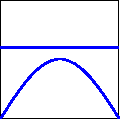
\includegraphics[]{Images/fig-bosonBC.pdf}

    \caption{Two possible views as the problem. We can constrain the bosons to a box of side length $L$ with hard boundaries, constraining the ground state wavefunction to look like $\sqrt{\frac{2}{L}}\sin(\frac{2\pi x}{L})$. Alteratively, we can assume our system is a finite patch out of infinite space, in which case the ground state wavefunctions are plane waves with infinite wavelength, i.e. constant in space.}
    \label{fig-bosonBC}
\end{figure}

In fact, the wavefunction and the energy would be quite sensitive to the boundary conditions. This is not something that we really want\footnote{as theorists in a QFT class, anyway; maybe not if you work at SBQMI down the street.}. We could do the opposite and remove the walls, and assume that our system is a finite patch within infinite space. Then a piece of the system should look fairly generic. But what happens then? The wavefunction would be constant over all space if $\v{k} = \v{0}$, so the probability of finding it anywhere in space is equal. So, our state is not something with a constant particle number. So at the outset, we can take this point of view that the particle number is not fixed; an approach that particle physicists and field theorists love. One could instead take a closed system and study it through this method, but there is not a consensus as to whether the two approaches are actually equivalent. But we will take the field theorists approach, here.

Motivated by this argument, we consider the state:
\begin{equation}
    \ket{\O} = \sum_{N=0}^\infty c_N\left(\alpha^\dag(\v{0})\right)^N \ket{0}.
\end{equation}
This is still not quite sensible; perhaps we can take something like:
\begin{equation}
    \alpha_f^\dag = \int d^3x f(\v{x})\alpha^{dag}(\v{k})
\end{equation}
for $f$ square integrable if we wanted to be a tad more rigorous, but let us not worry ourselves with this very much. How do we characterize such states? One thing we can notice is:
\begin{equation}
    \bra{\O}\psi(\v{x}, t)\ket{\O} \neq 0.
\end{equation}
The field operator annihilates a boson, but it will still have a nonzero overlap with the original vacuum state, so the overall expectation value will be nonzero (see HW2). Note that this is okay for bosons, but we would never see this for fermions. This is hugely degenerate if the bosons are non-interacting. 

\subsection{Coherent States}
Let us talk for a little about coherent states, which have the above expectation value property. At $t = 0$, we consider the field-operator commutation relations:
\begin{equation}
    [\psi(\v{x}), \psi^{\dag}(\v{y})] = \delta^{3}(\v{x} - \v{y})
\end{equation}
and:
\begin{equation}
    [\psi^\dag(\v{x}), \psi^{\dag}(\v{y})] =  [\psi(\v{x}), \psi(\v{y})] = 0.
\end{equation}
If we act the annhilation operator on the empty vacuum, we have:
\begin{equation}
    \psi(\v{x})\ket{0} = 0.
\end{equation}
We do not concern ourselves with the spin. Now, we consider the state:
\begin{equation}
    \ket{\eta} = e^{\int d^3x\left(\eta^*(\v{x})\psi(\v{x}) - \psi^\dag(\v{x})\eta(\v{x})\right)}\ket{0}
\end{equation}
where the operator in the exponential is anti-hermitian and so the overall operator is unitary. If we write the normal ordered version of the above, we obtain:
\begin{equation}
    \ket{\eta} = e^{-\int d^3x \eta^*(\v{x})\eta(\v{x})}e^{-\int d^3x \eta(\v{x})\psi^\dag(\v{x})}\ket{0}
\end{equation}
where we have got rid of the $\psi$ term by considering that this annhilates the vacuum state. We can write the action of the annihilation operator on the coherent state as:
\begin{equation}
    \psi(\v{x})\ket{\eta} = \eta(\v{x})\ket{\eta}.
\end{equation}
So that's a cool property! It's also a unitary transform of the vacuum state, so it is normalized:
\begin{equation}
    \braket{\eta}{\eta} = 1.
\end{equation}
So this is an example of the state where:
\begin{equation}
    \bra{\psi}\psi(\v{x})\ket{\eta} = \eta(\v{x}).
\end{equation}
This is an example of a ``good'' coherent state (as opposed to a bad one) and very often in physics we used bad ones. What could go wrong? For example, the integral $\int d^3x \eta^*(\v{x})\eta(\v{x})$ could diverge if $\eta(\v{x})$ is a constant. This often happens, actually (and we will proceed to work with this right now). The bad coherent state is ubiquotous; any interaction state of charges particles produces a ``coherent'' state of soft photons, but this is a bad coherent state (it has no overlap with any state which has a finite number of photons). Every QED interaction produces an infinite number of photons, which fly away undetected, but seem to be always there. So, we drop ``true/good'' coherent states for now, and work with bad ones; which will still give us sensible results.

\subsection{Landau's Argument for Superfluidity}
Note that in the textbook that there is a section which reviews Landau's famous argument about the quasiparticle spectrum and critical velocity of a superfluid. It uses Galilean symmetry, and so we don't cover it here (and the treatment of the book is so refined, that it is probably better to read it there). There is however the idea of a superfluid flowing through a pipe, without resistance, and so even if we introduce some interactions (between the particles, and with the pipe), it will flow through the pipe without any resistance. This is to some extent seen in the lab, and there is seen that if the superfluid goes too fast then the superfluid starts to feel resistance. Landau's argument goes as follows. For the energy to dissipate, there should be some excitations in the fluid. So, there should be some viscosity that creates a travelling wave/ripple (sometimes called quasiparticles) in the fluid. Let us say this is wavelike (everything is quantum mechanical here), with a wavenumber $\v{k}$ and frequency $\omega(\v{k})$. 

\begin{figure}[htbp]
    \centering
    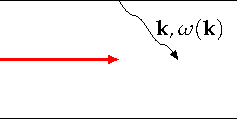
\includegraphics[]{Images/fig-superfluidpipe.pdf}

    \caption{In Landau's argument for superfluids, we consider a superfluid travelling in a pipe, and wavelike excitations/quasiparticles with wavenumber $\v{k}$ and frequency $\omega(\v{k})$.}
    \label{fig-superfluidpipe}
\end{figure}


He then argues that this should be energetically favourable if the velocity is larger than a critical velocity $v_c$:
\begin{equation}
    v_c = \min_\v{k} \frac{\omega(\v{k})}{\abs{\v{k}}}.
\end{equation}
The argument is beautiful in how it invokes Galilean relativity/symmetry (do read about it in your own time!) Note the stark difference from the free particle case; as then we would have $\omega(\v{k}) \propto \v{k}^2$ so $v_c = 0$, i.e. free particles are not superfluidic. What does work is if we have a sound wave, as then $\omega(\v{k}) = v_s\abs{\v{k}}$; here the critical velocity is the speed of sound.

So, the important goal for us; can we find this using our model? What do the elementary excitations look like?

A small aside; this argument doesn't really agree with experiments. $v_c$ as measured is smaller than what we would expect from Landau's argument. The explanation is that the dispersion relation $\omega(\v{k})$ as measured in experiment takes the form of the roton curve as seen in the below figure. Then $v_c$ is not the slope of the purple curve (as would be predicted theoretically) but instead is the slope of the red curve (less than the theoretically predicted value).

\begin{figure}[htbp]
    \centering
    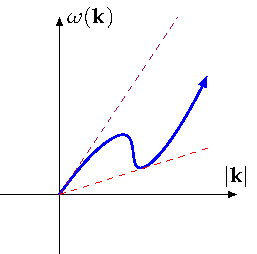
\includegraphics[]{Images/fig-rotoncurve.pdf}

    \caption{Plot of the experimental dispersion relation for superfluids (roton dispersion relation). From this we can see the reason for the experimental disagreement of the Landau argument for determining the critical velocity $v_c$ of superfluids, as the local minimum in the roton curve shifts the critical velocity to be the slope of the red curve, rather than the Landau theoretical prediction of the purple curve.}
    \label{fig-rotoncurve}
\end{figure}

\subsection{Introducing a Small Interaction to our QFT}
We introduce a weak repulsive interaction between the bosons that supresses the Bose-Einstein condensation. They will want to be far apart and run away from our system; so we add a chemical potential to balance this and draw them back in (so we end up with a finite density at the end). Let us write down a Hamiltonian\footnote{A remark: model building is often much easier than the actual toying with the (e.g. field) equations...} for this:
\begin{equation}
    H = \int d^3 x \left(\frac{\hbar^2}{2m}\nabla \psi^\dag(\v{x}) \cdot \nabla \psi(\v{x}) - \mu\psi^{\dag}(\v{x})\psi(\v{x}) + \frac{\lambda}{2}\psi^\dag(\v{x})\psi^{\dag}(\v{x})\psi_\v{x}\psi(\v{x})\right)
\end{equation}
where the last term is a ball-bearing potential, with $\lambda$ ``small'' (and positive; else the spectrum will not be bounded from below, as the energy from all the particles sitting on top of each other will be negative infinity). We also enforce the commutation relations:
\begin{equation}
    [\psi(\v{x}, t), \psi^{\dag}(\v{y}, t)] = \delta^3(\v{x} - \v{y}), \quad [\psi^\dag(\v{x}, t), \psi^{\dag}(\v{y}, t)] = [\psi(\v{x}, t), \psi(\v{y}, t)] = 0
\end{equation}
and also introduce the vacuum state $\ket{\O}$, which is the lowest-eigenvalue eigenstate of the (bounded-from-below) Hamiltonian. It is possible that the expectation value is nonvanishing, so let us anticipate this and introduce a function $\eta(\v{x})$:
\begin{equation}
    \bra{\O}\psi(\v{x}, t)\ket{\O} = \eta(\v{x}) \neq 0.
\end{equation}

How do we treat this possibility in a systematic way? One way would be to write:
\begin{equation}
    \psi(\v{x}, t) = \eta(\v{x}, t) + \tilde{\psi}(\v{x}, t)
\end{equation}
where $\eta$ is the classical part and $\tilde{\psi}$ is the quantum/non-classical part, i.e. which follows:
\begin{equation}
    \bra{\O}\tilde{\psi}(\v{x}, t)\ket{\O} = 0.
\end{equation}
So, there will be a classical part of the Hamiltonian where we forget about the $\tilde{\psi}$s, and in this term we would like $\eta$s which minimize the Hamiltonian. Then we can solve a classical field equation, check the extremum of the functional etc. We can argue that the $\eta$ that minimizes the Hamiltonian goes as:
\begin{equation}
    \eta \sim \frac{1}{\sqrt{\lambda}}.
\end{equation}
At very weak coupling, this classical piece is emphasized. We then might ask what the size of the quantum part is. Since $\psi$ needs to obey equal-time commutation relations, and $\eta$ drops out of these (as it is classical and drops out of the commutation relations), then since $\tilde{\psi}$ follows the commutation relations (where $\lambda$ shows up nowhere), this tells us that $\tilde{\psi}$ is of order unity:
\begin{equation}
    \tilde{\psi} \sim \lambda^0 = 1.
\end{equation}
If we make $\lambda$ small, we can then ignore anything but the classical $\eta$ term. We can consider an asymptotic expansion of $\eta$ (asymptotic as the first term is singular) and $\tilde{\psi}$, each of which have corrections which can be solved order by order. This is an arbitrarily good approach so long as $\lambda$ is arbitrary small and nonzero. Let us take it (next class!)

Another thing we might be interested in is the ``smoothest'' possible states, i.e. states that have some symmetry. A smooth surface has translation symmetry. We expect that the low-energy states of our theory here may be smooth. Suppose $\eta$ was a constant; then the most important part of our field is smooth. This is like going back to our condensate at the start of our lecture, where our wavefunctions were constant throughout all space. We then simply search for a constant which minimizes the Hamiltonian. The kinetic energy terms are zero if $\eta$ is a constant, and we can minimize the other terms to find:
\begin{equation}
    \eta = \sqrt{\frac{\mu}{\lambda}} \sim \frac{1}{\sqrt{\lambda}}.
\end{equation}
From our theory we can calculate the density:
\begin{equation}
    \rho \cong \frac{\mu}{\lambda}
\end{equation}
and the (grand canonical free) energy:
\begin{equation}
    \Phi = -\frac{\mu^2}{2\lambda} + \ldots = -\frac{\lambda}{2} \rho^2 + \ldots
\end{equation}
which is also equal to the negative of the pressure:
\begin{equation}
    P = -\Phi = \frac{\lambda}{2}\rho^2.
\end{equation}
So already this theory gives us a lot to work with, but we have yet to show that it is in fact a superfluid; this is something we will calculate and verify next class, by figuring out what $\omega(\v{k})$ is for our theory. 